\documentclass{beamer}
\usepackage{amsfonts,amsmath,oldgerm}
\usetheme{_statale}
\usefonttheme[onlymath]{serif}

\usepackage{enumitem}
\usepackage[italian]{babel}
\usepackage{xcolor}
\usepackage{graphicx}

\usepackage{hyperref}
\newcommand{\hypercite}[2]{\href{#1}{\cite{#2}}}

\usepackage[backend=biber, style=authoryear]{biblatex}
\addbibresource{bibliografia.bib}

%\newcommand{\testcolor}[1]{\colorbox{#1}{\textcolor{#1}{test}}~\texttt{#1}}
%\newcommand{\hrefcol}[2]{\textcolor{cyan}{\href{#1}{#2}}}
\titlebackground*{assets/background}

\renewcommand{\figurename}{Figura}


\title{Ghiacciaio del Morteratsch}
\course{Glaciologia e Climatologia Alpina}
\author{Filippo Negrini}
\IDnumber{Matricola: 47127A}
\date{}


\begin{document}
\maketitle


\section{Introduzione}


\begin{frame}
    \frametitle{Morteratsch in numeri}
    \framesubtitle{}

    \begin{columns}
        \begin{column}{0.5\textwidth}
            \begin{itemize}[itemsep=0.5em, label=$\bullet$]
                \item Superficie: 14.93 km$^2$
                \item Volume: 0.899 km$^3$
                \item Quota fronte: 2117 m
                \item Quota massima: 4049 m
                \item Spessore medio: 61.4 m
                \item Spessore massimo: 280.7 m
            \end{itemize}
            \vspace{12pt}

            Dati da \hypercite{https://doi.glamos.ch/pubs/glrep/glrep_141-142.html}{GLAMOS22}
        \end{column}
        
        \begin{column}{0.5\textwidth}
        \begin{figure}
            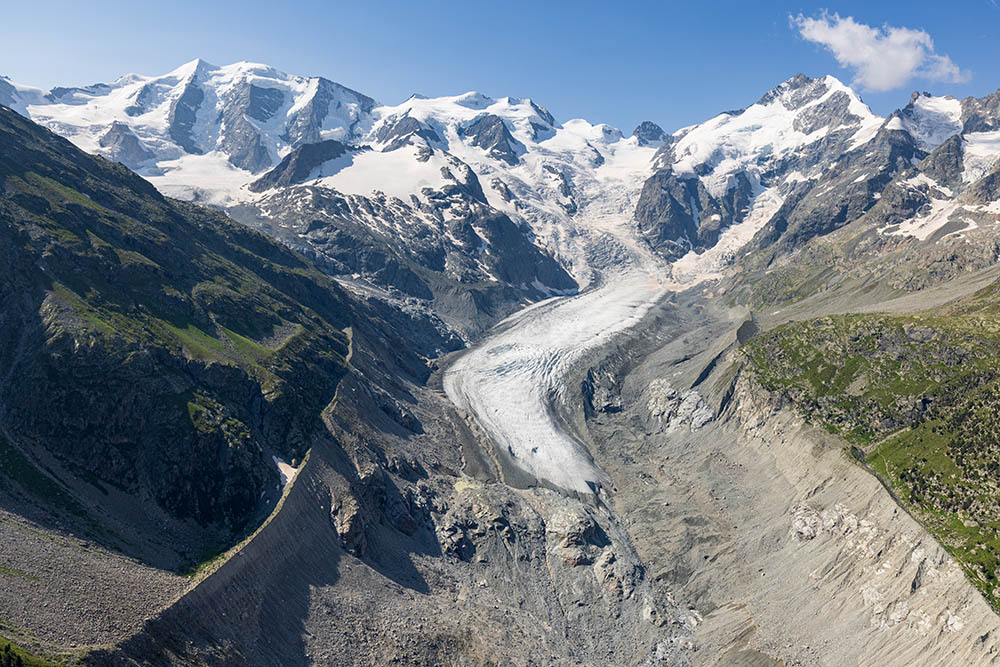
\includegraphics[width=0.8\textwidth]{Immagini/AereaMorteratsch.jpg}
            \caption{Foto da \href{https://www.swisseduc.ch/glaciers/morteratsch/2021/index-en.html}{\textcolor{blue}{SwissEduc}}}
          \end{figure}
        \end{column}
      \end{columns}
  
\end{frame}


\begin{frame}
  \frametitle{Confronto}
  \framesubtitle{}
  
  \begin{figure}
    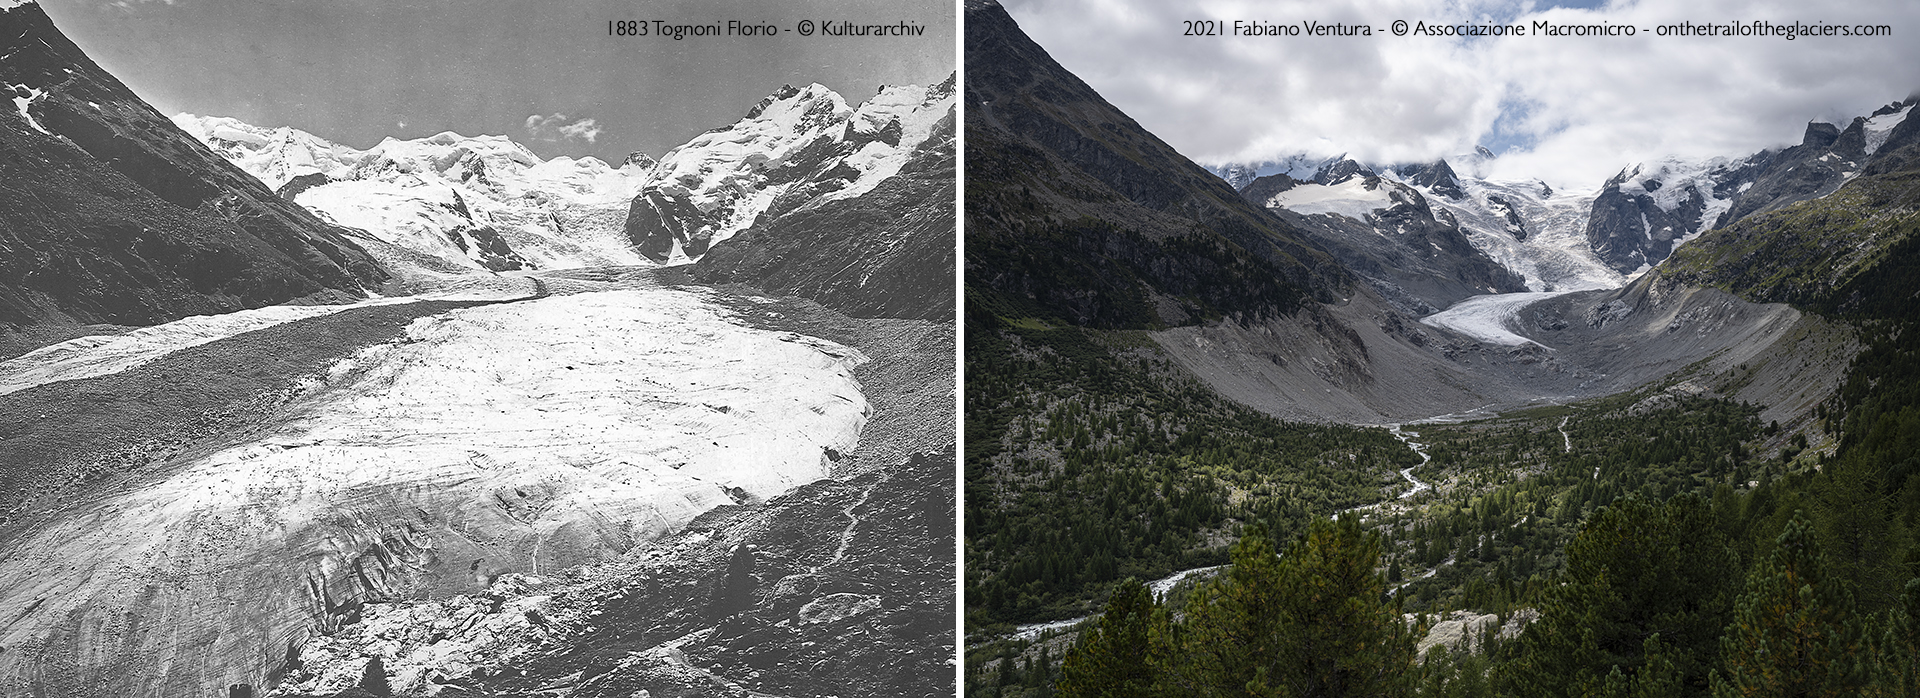
\includegraphics[width=\textwidth]{Immagini/ConfrontoMorteratsch.jpg}
    \caption{Ghiacciaio del Morteratsch nel 1883 e nel 2021. (Fabiano Ventura - 2021)}
  \end{figure}

\end{frame}

\begin{frame}
  \frametitle{Vadret Pers}
  \framesubtitle{}

  \begin{columns}
      \begin{column}{0.5\textwidth}
          \begin{itemize}[itemsep=0.5em, label=$\bullet$]
              \item Separato dal Morteratsch nel 2017
              \item Superficie: 6.7 km$^2$
              \item Quota minima: 2450 m
              \item Quota massima: 3900 m
          \end{itemize}
          \vspace{12pt}

          Dati da \hypercite{https://doi.glamos.ch/pubs/glrep/glrep_141-142.html}{GLAMOS22}
      \end{column}
      
      \begin{column}{0.5\textwidth}
      \begin{figure}
          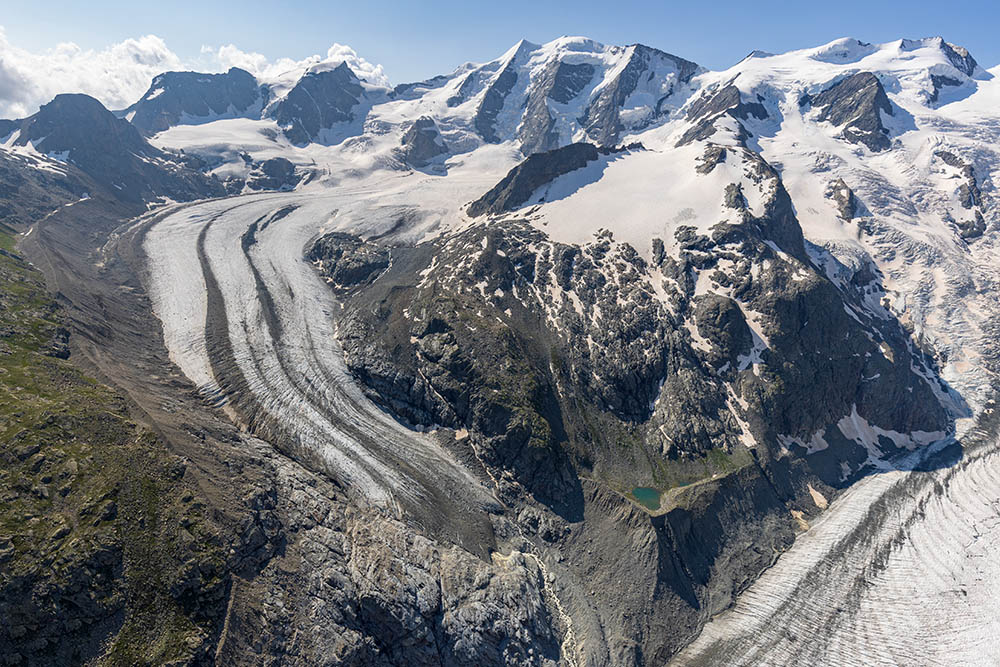
\includegraphics[width=0.8\textwidth]{Immagini/vadretPers.jpg}
          \caption{Foto da \href{https://www.swisseduc.ch/glaciers/morteratsch/2021/index-en.html}{\textcolor{blue}{SwissEduc}}}
        \end{figure}
      \end{column}
    \end{columns}

\end{frame}
\section{Analisi}


\begin{frame}
    \frametitle{Variazioni frontali}
    \framesubtitle{}

    \begin{figure}
        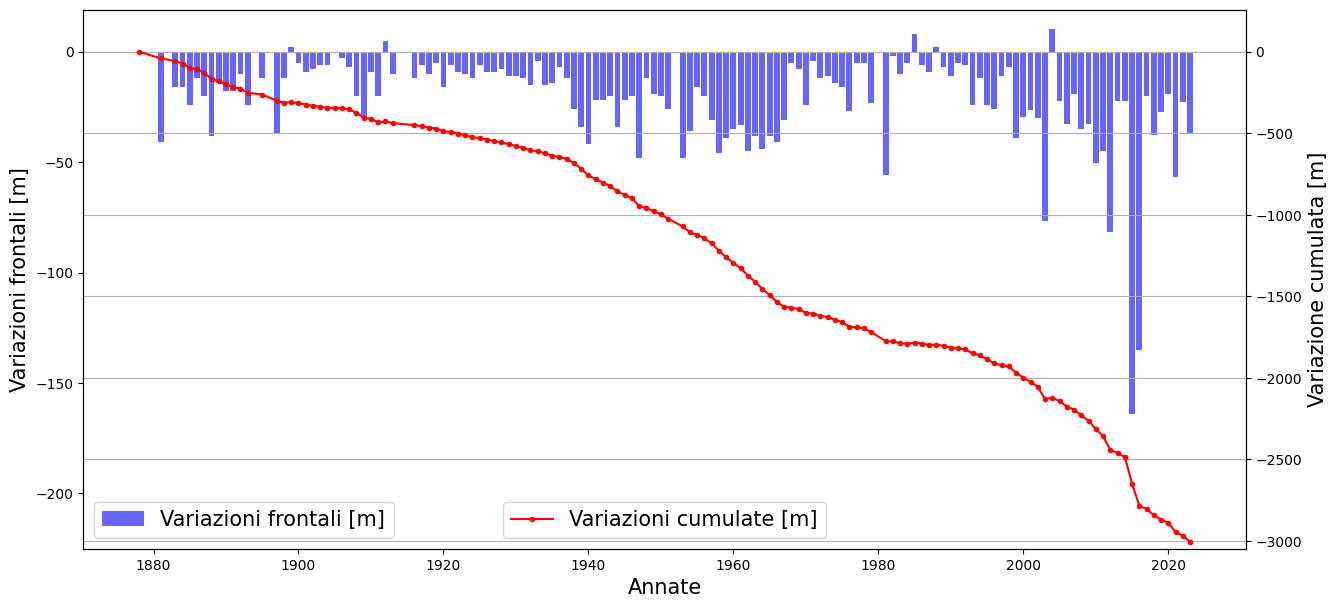
\includegraphics[width=0.9\textwidth]{Immagini/variazioniSovrapposte.png}
        \caption{Dati da \cite{GLAMOS23}}
    \end{figure}
  
\end{frame}


\begin{frame}
    \frametitle{Ablation stakes Morteratsch}
    \framesubtitle{}

    \begin{figure}
        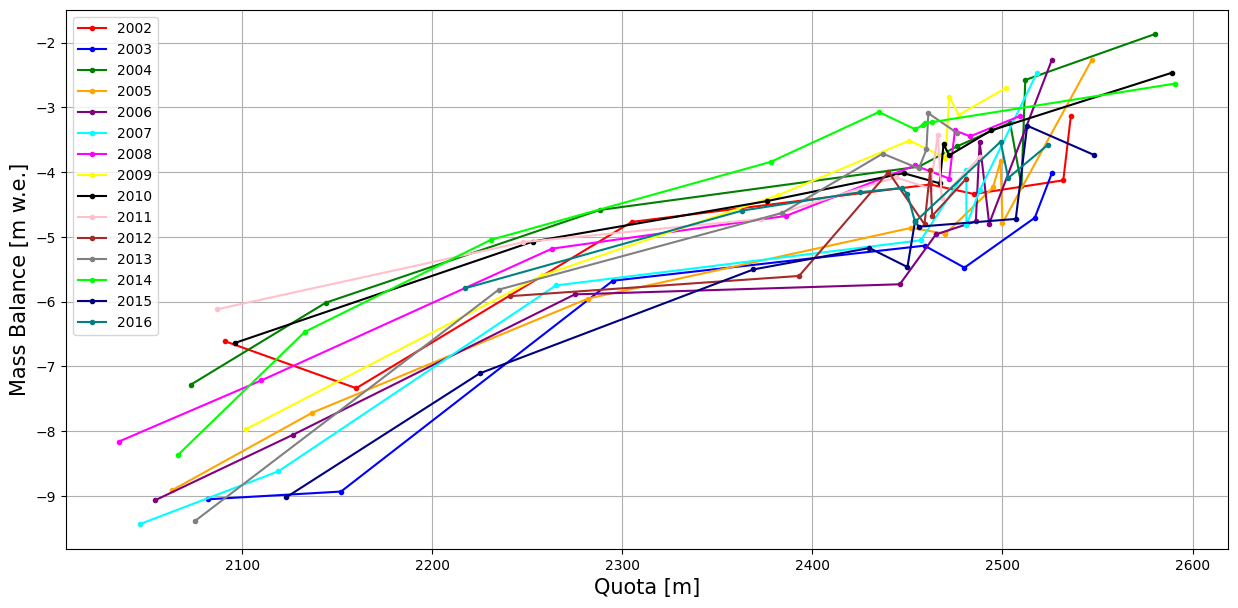
\includegraphics[width=0.9\textwidth]{Immagini/annateMassBalanceMorteratsch.png}
        \caption{Dati da \cite{STAT2018}}
    \end{figure}
  
\end{frame}


\begin{frame}
    \frametitle{Ablation stakes Vadret Pers}
    \framesubtitle{}

    \begin{figure}
        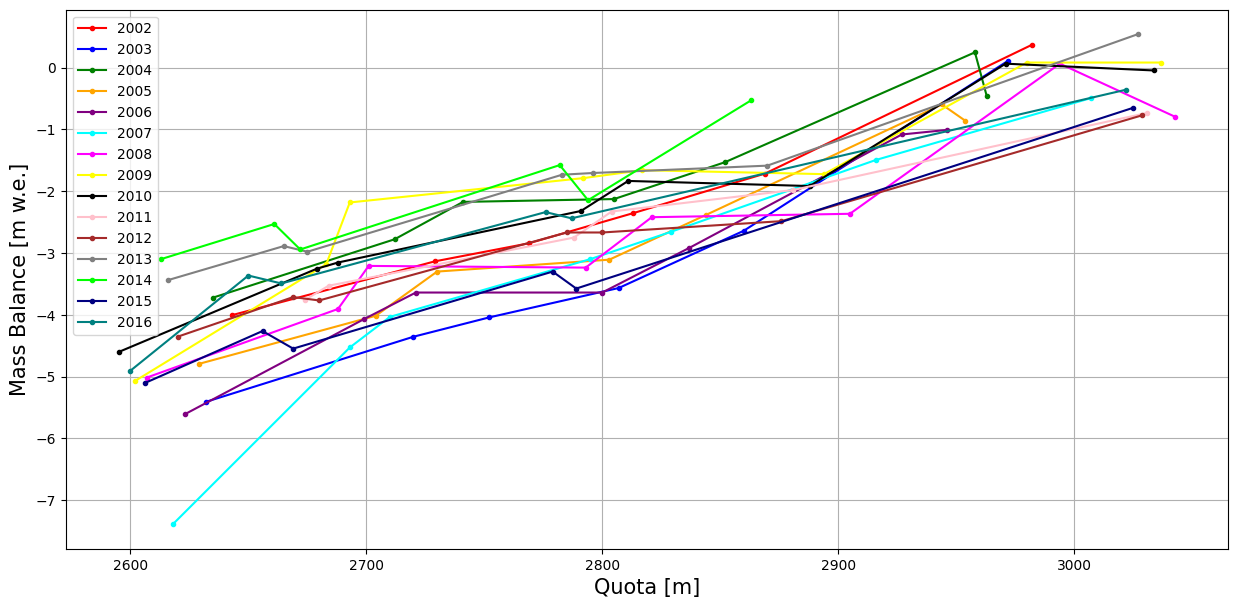
\includegraphics[width=0.9\textwidth]{Immagini/annateMassBalanceVadretPers.png}
        \caption{Dati da \cite{STAT2018}}
    \end{figure}
  
\end{frame}


\begin{frame}
    \frametitle{ELA Vadret Pers}
    \framesubtitle{}

    \begin{figure}
        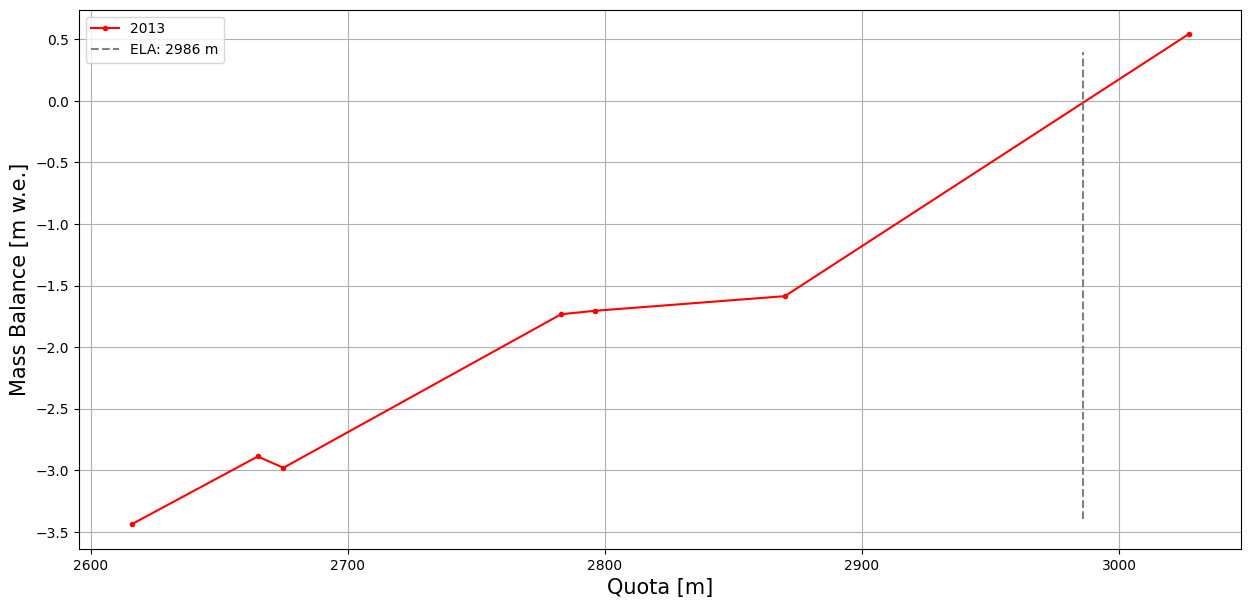
\includegraphics[width=0.9\textwidth]{Immagini/elaPers.png}
        \caption{Dati da \cite{STAT2018}}
    \end{figure}
  
\end{frame}


\begin{frame}
    \frametitle{AWS Morteratsch}
    \framesubtitle{}

    \begin{figure}
        \includegraphics[width=0.55\textwidth]{Immagini/awsMorteratsch2018.png}
        \caption{Foto da \href{https://www.projects.science.uu.nl/iceclimate/aws/alpine.php}{\textcolor{blue}{IMAU}}}
    \end{figure}
  
\end{frame}


\begin{frame}
    \frametitle{Shortwave radiation}
    \framesubtitle{}

    \begin{figure}
        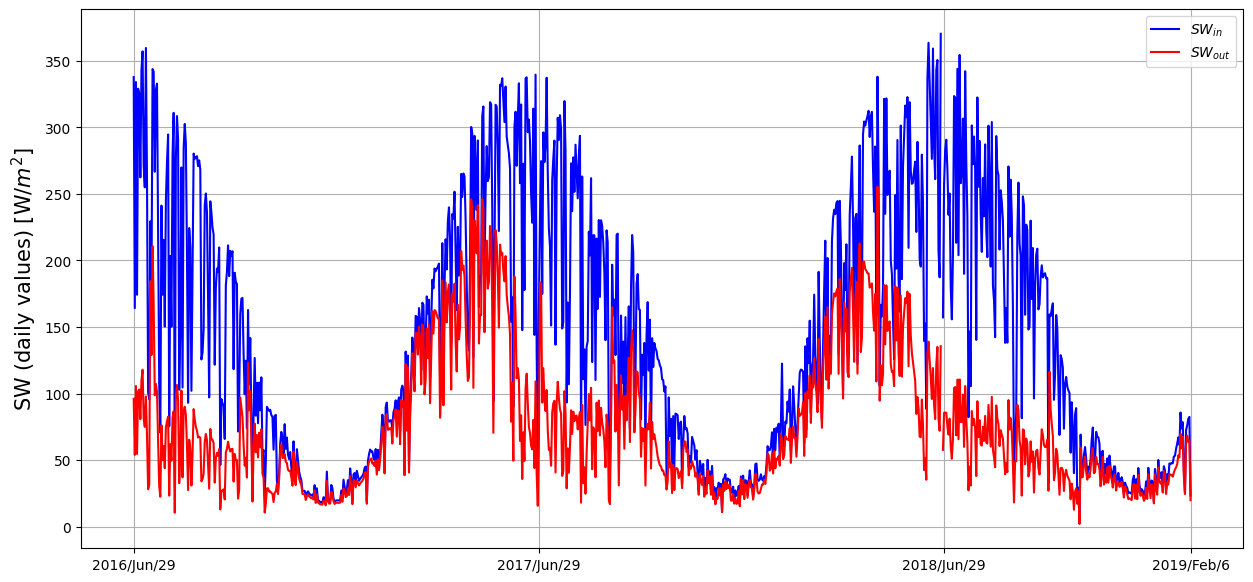
\includegraphics[width=0.9\textwidth]{Immagini/shortWaveDaily.png}
        \caption{Dati da Oerlemans}
    \end{figure}
  
\end{frame}


\begin{frame}
    \frametitle{Albedo}
    \framesubtitle

    \center
    \begin{minipage}{0.5\textwidth}
        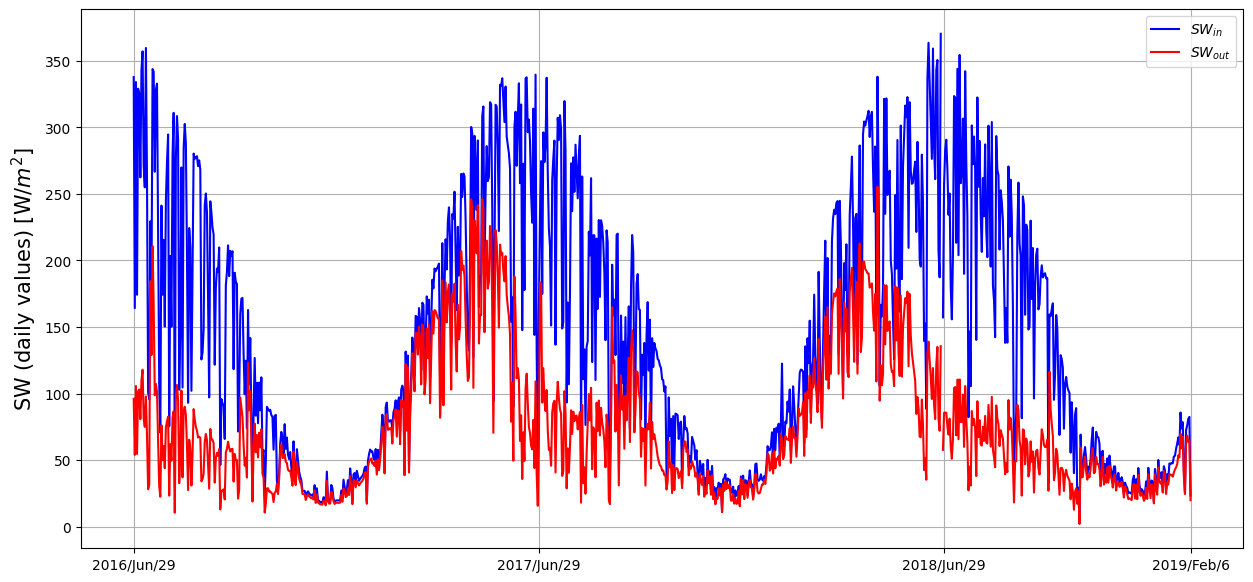
\includegraphics[width=\textwidth]{Immagini/shortWaveDaily.png}
    \end{minipage}
    \begin{minipage}{0.5\textwidth}
        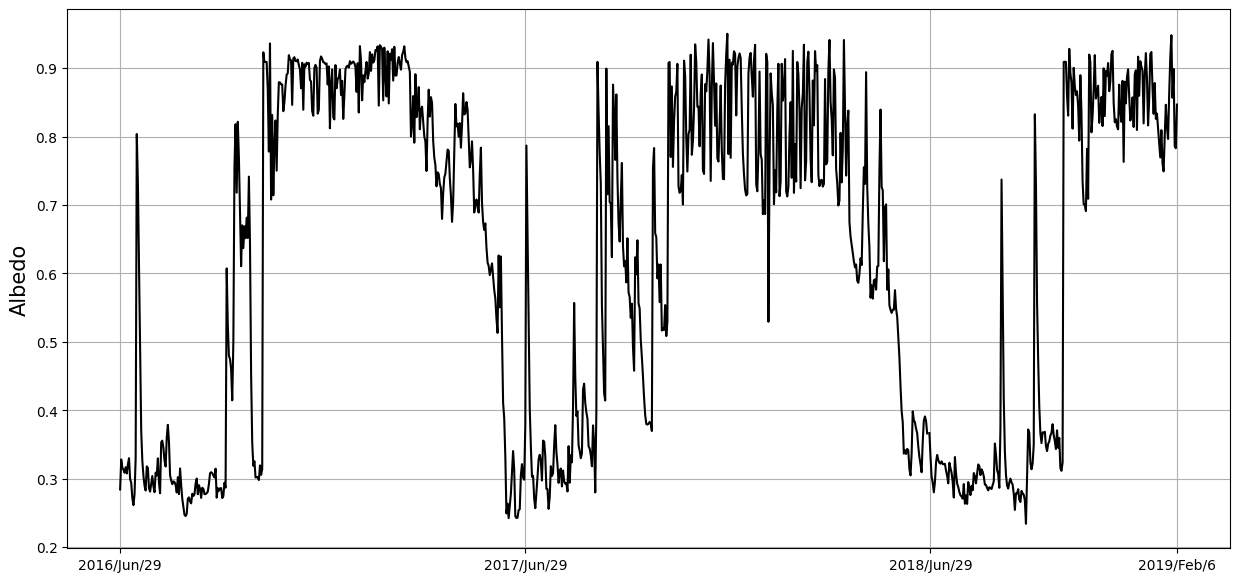
\includegraphics[width=\textwidth]{Immagini/albedoYear.png}
    \end{minipage}

\end{frame}

\begin{frame}
    \frametitle{Albedo per year}
    \framesubtitle

    \center
    \begin{figure}
        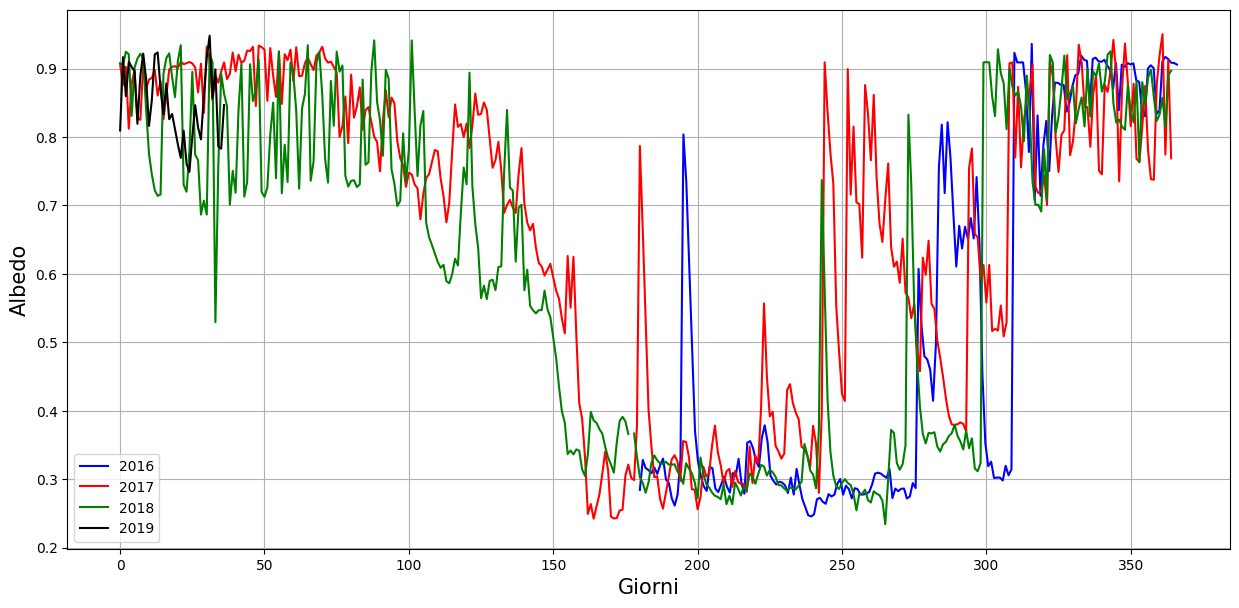
\includegraphics[width=0.9\textwidth]{Immagini/albedoPerYear.png}
        \caption{Dati da Oerlemans}
    \end{figure}

\end{frame}


\begin{frame}
    \frametitle{Longwave radiation}
    \framesubtitle{}

    \begin{figure}
        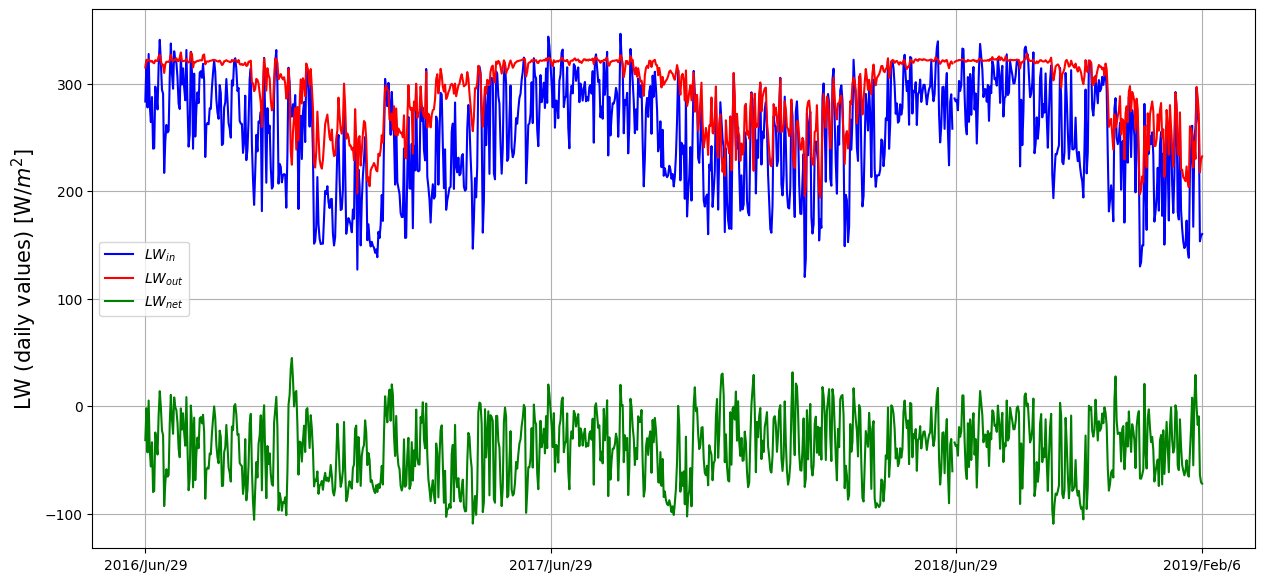
\includegraphics[width=0.9\textwidth]{Immagini/longWaveDaily.png}
        \caption{Dati da Oerlemans}
    \end{figure}
  
\end{frame}


\begin{frame}
    \frametitle{Total energy budget}
    \framesubtitle{}

    \begin{figure}
        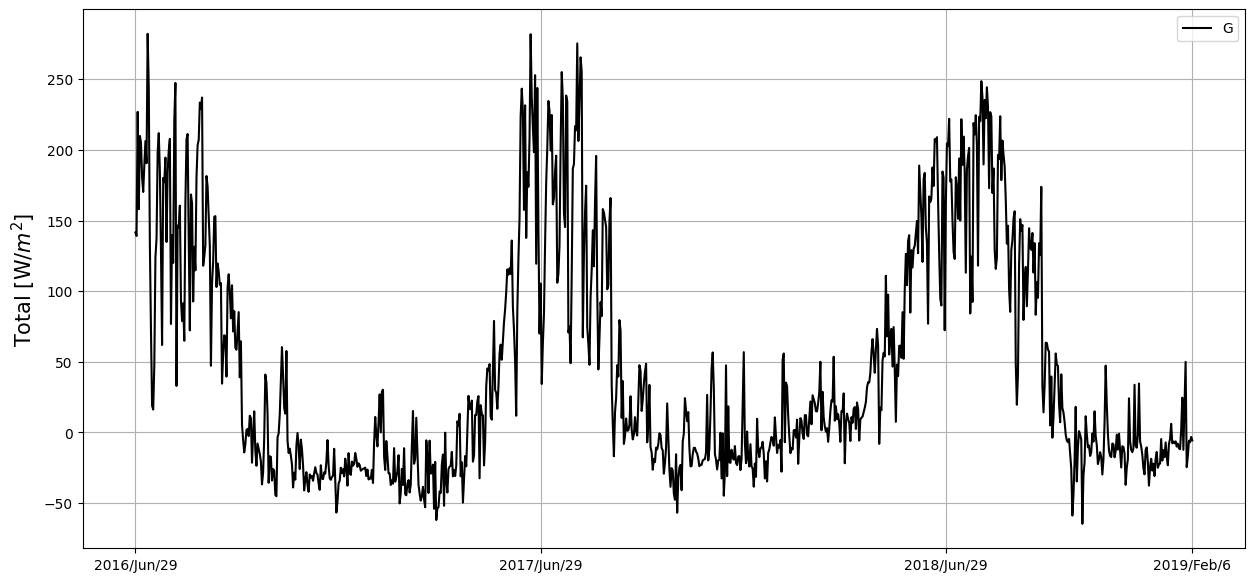
\includegraphics[width=0.9\textwidth]{Immagini/totalEnergy.png}
        \caption{Dati da Oerlemans}
    \end{figure}
  
\end{frame}


\begin{frame}
    \frametitle{Benchmark}
    \framesubtitle{}

    \begin{columns}
        
        \begin{column}{0.5\textwidth}
            \begin{figure}
                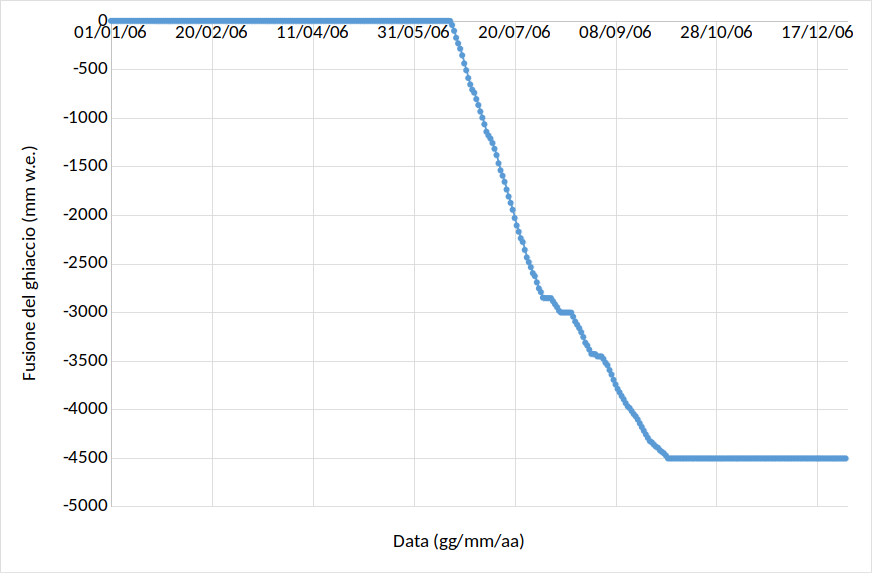
\includegraphics[width=\textwidth]{Immagini/forniLez.png}
            \end{figure}
        \end{column}
        
        \begin{column}{0.5\textwidth}
            \begin{figure}
                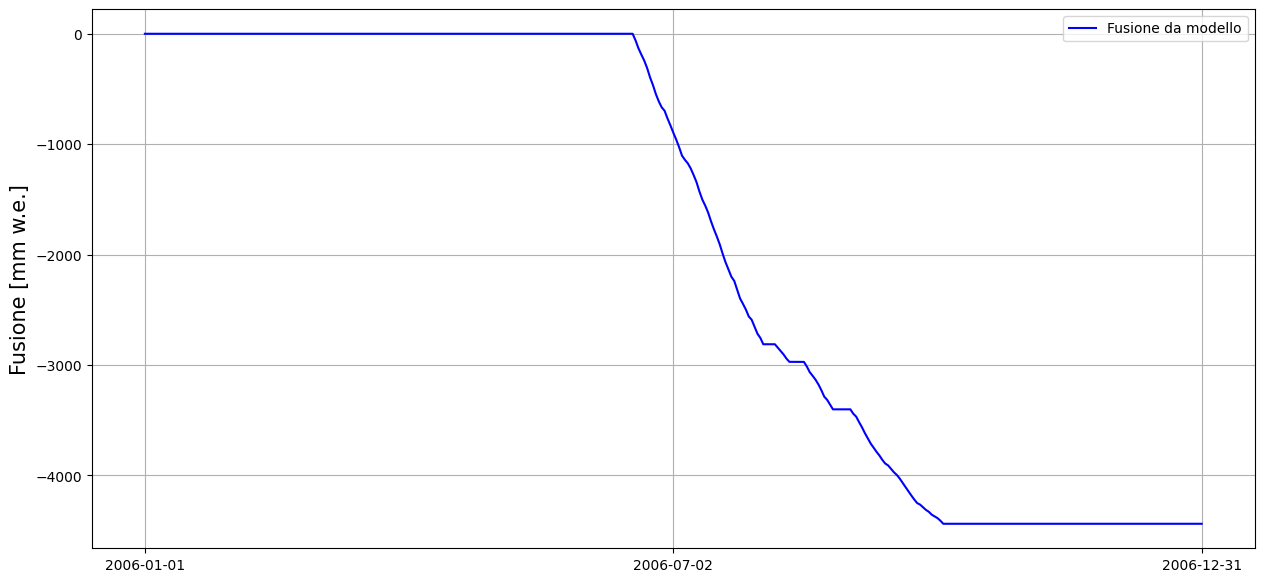
\includegraphics[width=\textwidth]{Immagini/forniBen.png}
            \end{figure}
        \end{column}
      \end{columns}
  
\end{frame}


\begin{frame}
    \frametitle{Melt}
    \framesubtitle{}

    \begin{figure}
        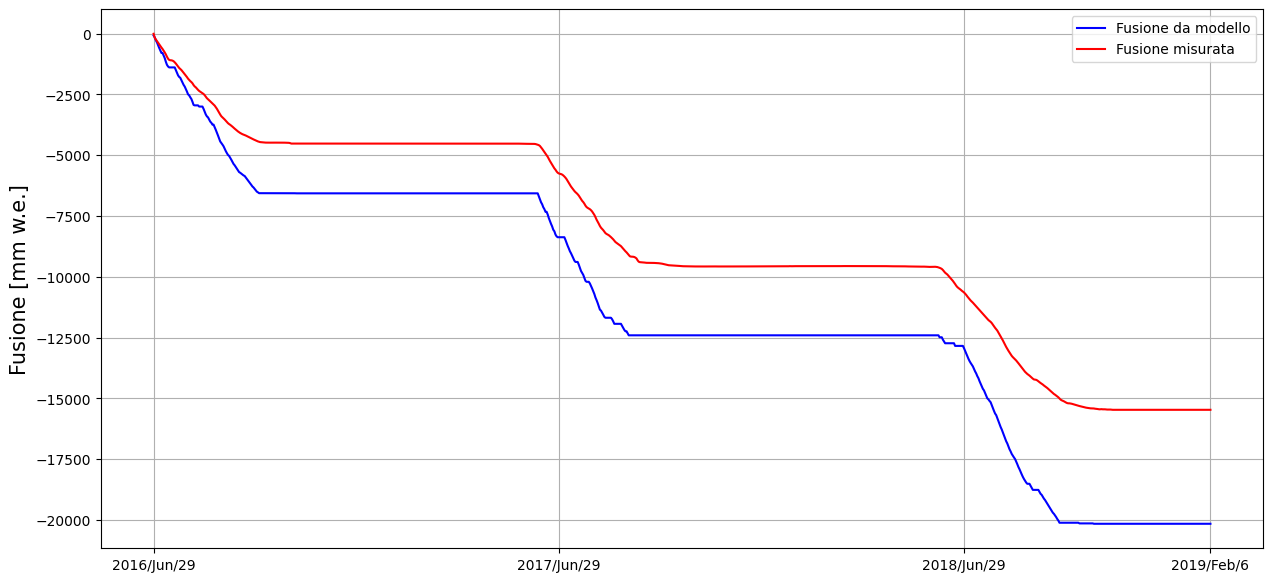
\includegraphics[width=0.9\textwidth]{Immagini/confrontoMelt.png}
        \caption{Dati da Oerlemans}
    \end{figure}
  
\end{frame}

\section{Confronto}


\begin{frame}
    \frametitle{Daily albedo values}
    \framesubtitle{}

    \center
    \begin{minipage}{0.5\textwidth}
        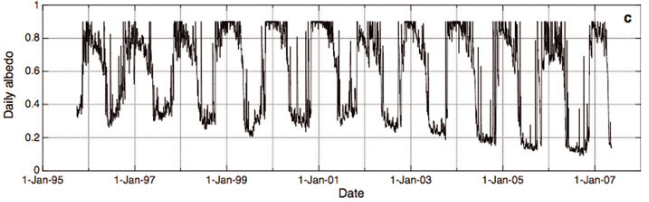
\includegraphics[width=\textwidth]{Immagini/albedoOerlemans.png}
    \end{minipage}
    \begin{minipage}{0.5\textwidth}
        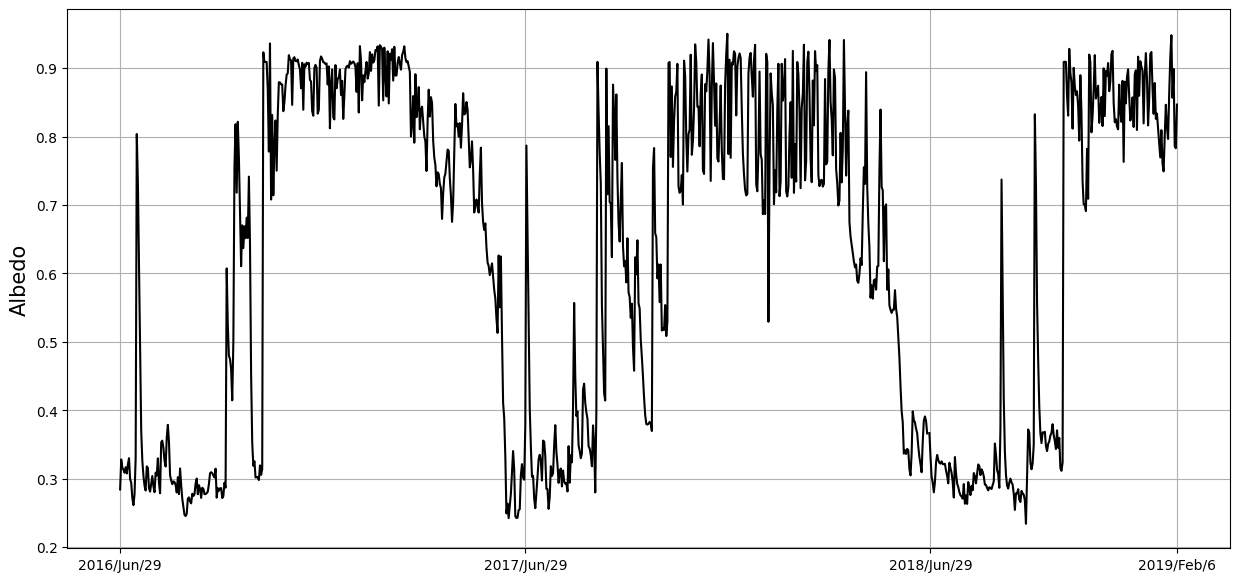
\includegraphics[width=\textwidth]{Immagini/albedoYear.png}
    \end{minipage}

\end{frame}


\begin{frame}
    \frametitle{Daily temperature values}
    \framesubtitle{}

    \center
    \begin{minipage}{0.5\textwidth}
        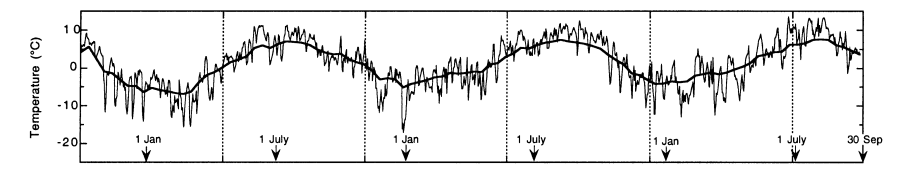
\includegraphics[width=\textwidth]{Immagini/temperaturaOerlemans.png}
    \end{minipage}
    \begin{minipage}{0.5\textwidth}
        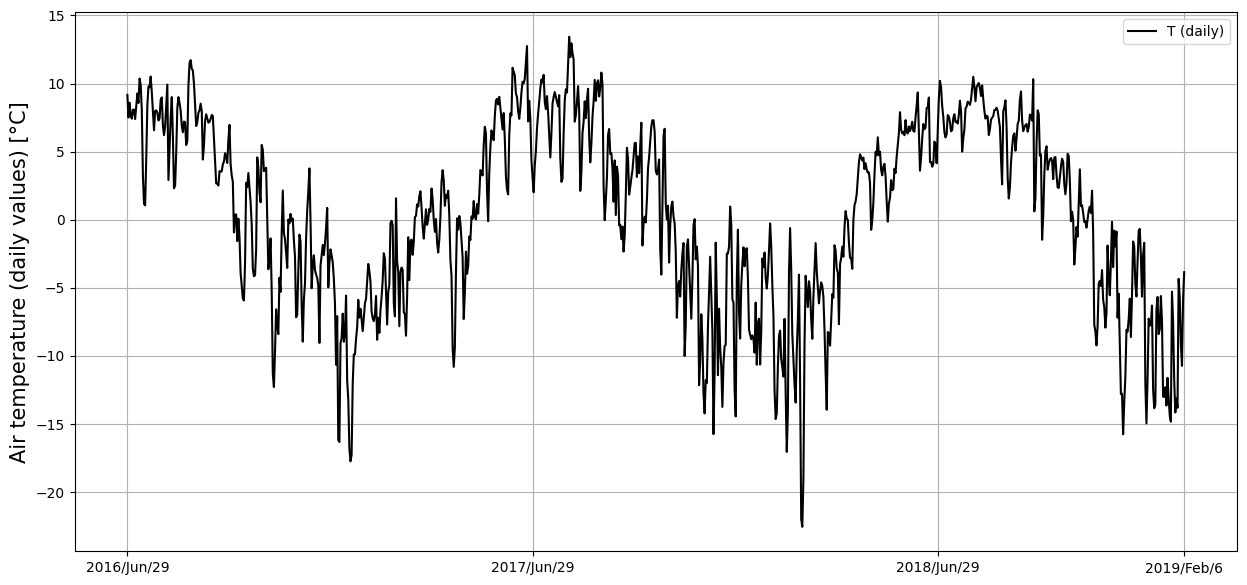
\includegraphics[width=\textwidth]{Immagini/tempAria.png}
    \end{minipage}

\end{frame}

\section{Conclusioni}

\begin{frame}

    \frametitle{Conclusioni}
    \framesubtitle{}
  
  \begin{itemize}[itemsep=1.5em, label=$\bullet$]
      \item Ritiro frontale di 3005 metri dall'inizio delle misurazioni
      \item Perdita di circa 5 m w.e. nei pressi del fronte glaciale
      \item Tendenza all'aumento della temperatura dell'aria a parità di quota
    \end{itemize}
  
  \end{frame}

\begin{frame}
    \frametitle{Fine}
    \framesubtitle{}

    \begin{center}
        Grazie per l'attenzione
    \end{center}
    
\end{frame}

\begin{frame}
    \frametitle{Bibliografia}
    \framesubtitle{}

    \begin{figure}
        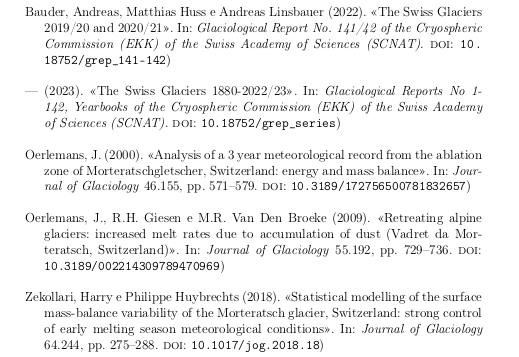
\includegraphics[width=0.6\textwidth]{Immagini/bibliografia.png}
    \end{figure}
    
\end{frame}
\section{Backup}


\begin{frame}
    \frametitle{Variazioni frontali}
    \framesubtitle{}

    \begin{figure}
        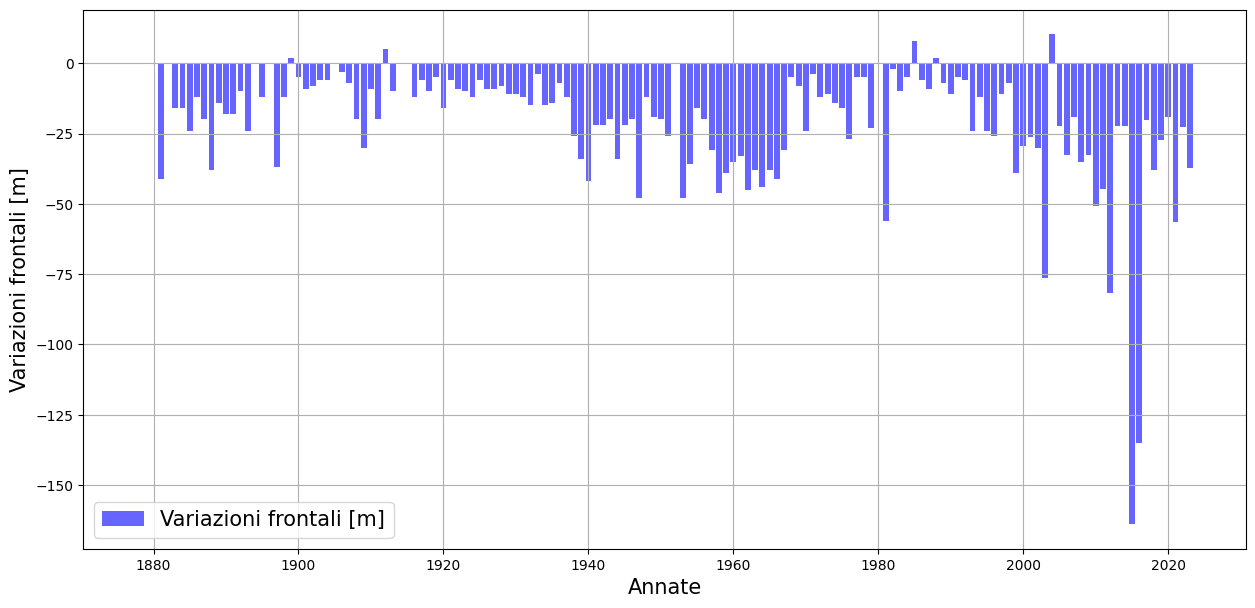
\includegraphics[width=0.9\textwidth]{Immagini/variazioniFrontali.png}
        \caption{Dati da \cite{GLAMOS23}}
    \end{figure}
  
\end{frame}


\begin{frame}
    \frametitle{Variazioni cumulate}
    \framesubtitle{}

    \begin{figure}
        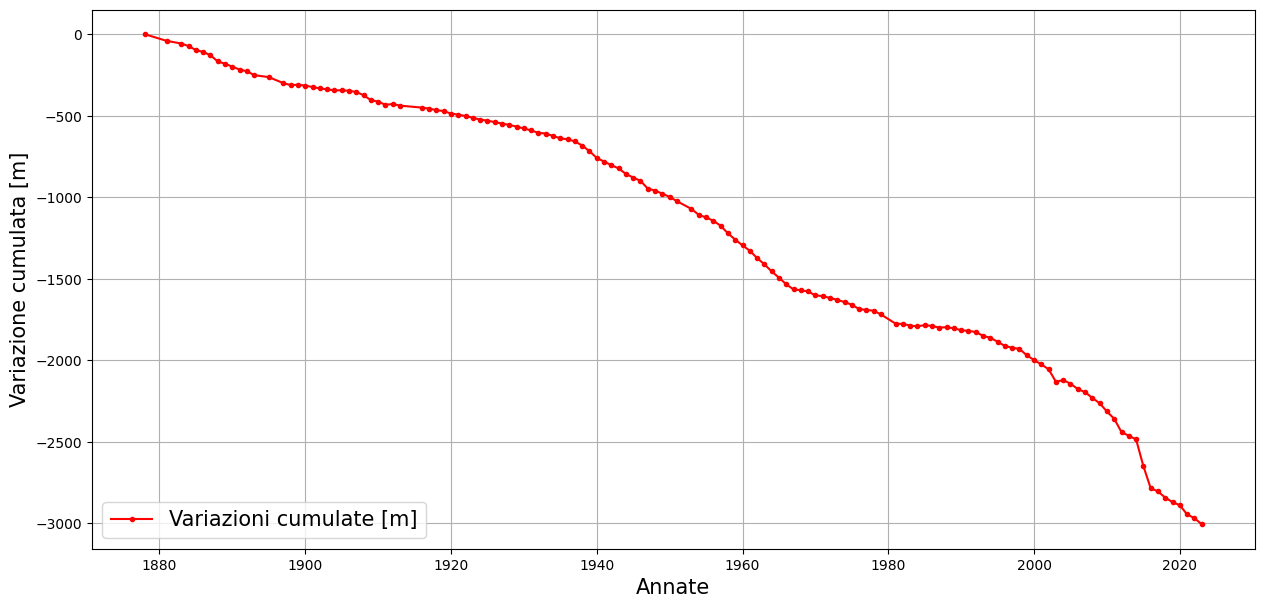
\includegraphics[width=0.9\textwidth]{Immagini/variazioniCumulative.png}
        \caption{Dati da \cite{GLAMOS23}}
    \end{figure}
  
\end{frame}


\begin{frame}
    \frametitle{Short-wave radiation}
    \framesubtitle{}

    \begin{figure}
        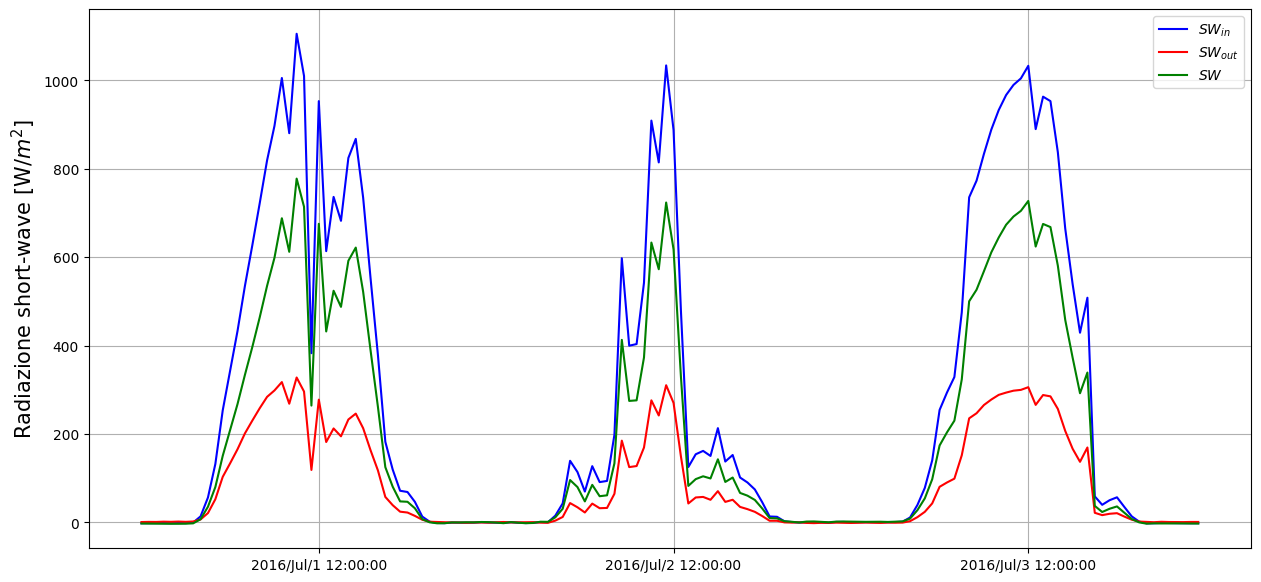
\includegraphics[width=0.9\textwidth]{Immagini/shortWave.png}
        \caption{Dati da Oerlemans}
    \end{figure}
  
\end{frame}


\begin{frame}
    \frametitle{Long-wave radiation}
    \framesubtitle{}

    \begin{figure}
        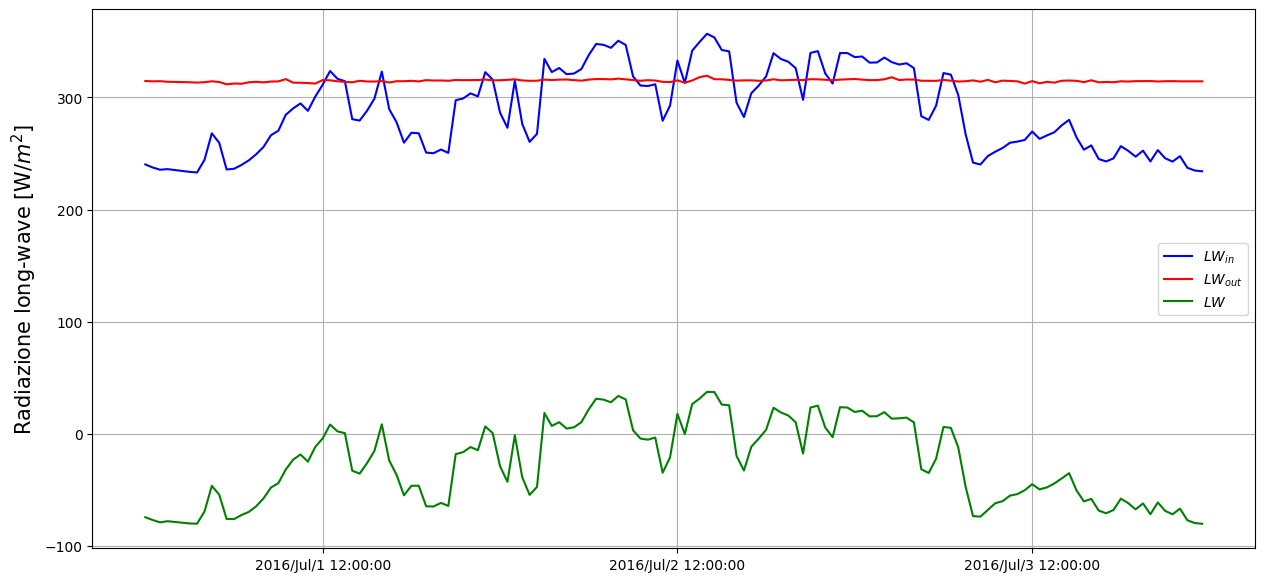
\includegraphics[width=0.9\textwidth]{Immagini/longWave.png}
        \caption{Dati da Oerlemans}
    \end{figure}
  
\end{frame}


\begin{frame}
    \frametitle{Albedo}
    \framesubtitle{}

    \begin{figure}
        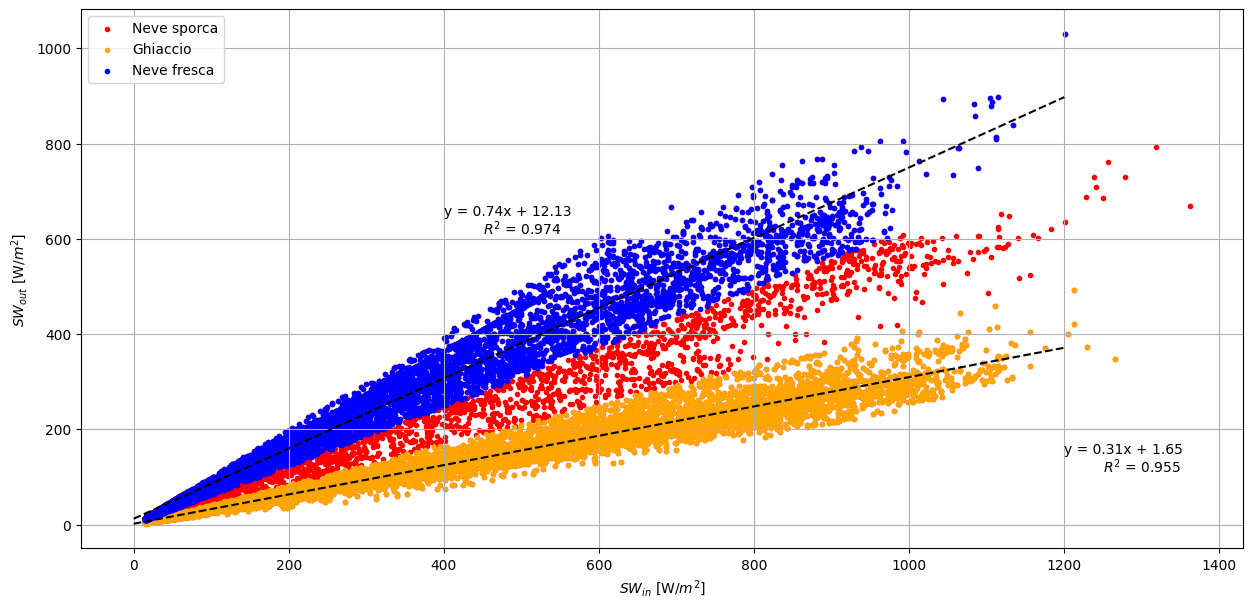
\includegraphics[width=0.9\textwidth]{Immagini/albedoHour.png}
        \caption{Dati da Oerlemans}
    \end{figure}
  
\end{frame}


\begin{frame}
    \frametitle{Temperatura}
    \framesubtitle{}

    \begin{figure}
        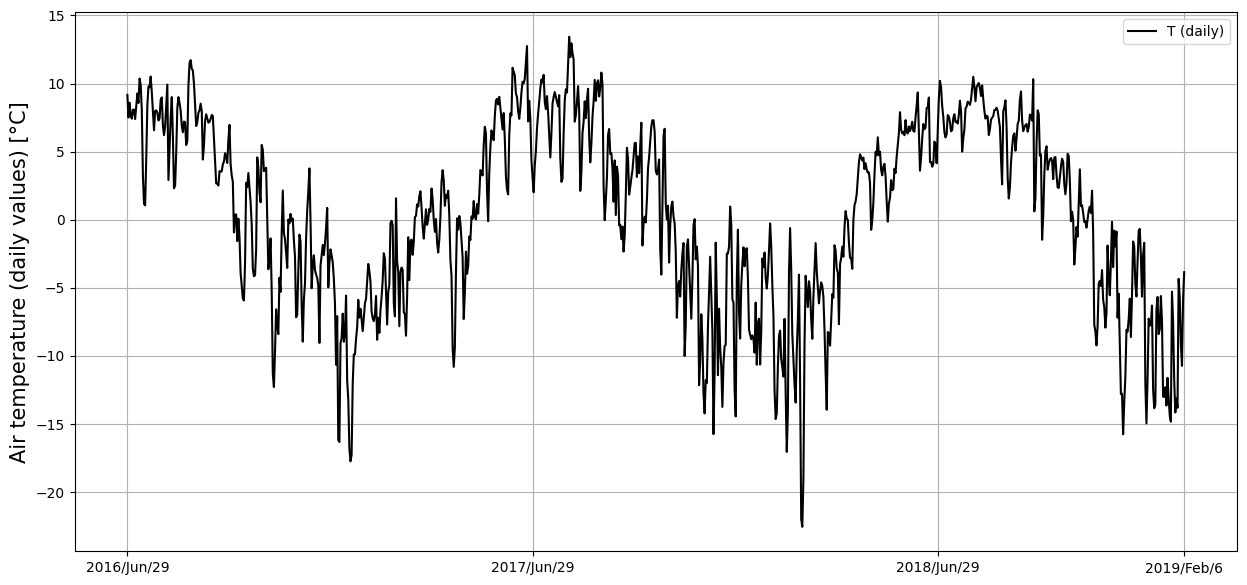
\includegraphics[width=0.9\textwidth]{Immagini/tempAria.png}
        \caption{Dati da Oerlemans}
    \end{figure}
  
\end{frame}


\begin{frame}
    \frametitle{Temperatura superficiale}
    \framesubtitle{}

    \begin{figure}
        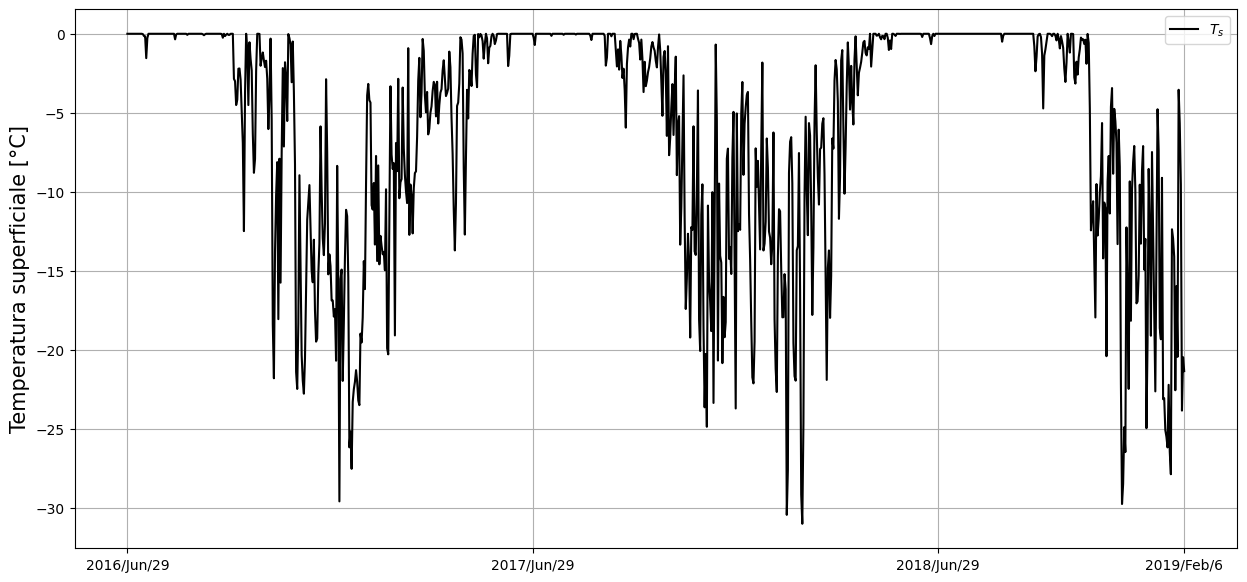
\includegraphics[width=0.9\textwidth]{Immagini/temperaturaYear.png}
        \caption{Dati da Oerlemans}
    \end{figure}
  
\end{frame}


\begin{frame}
    \frametitle{Sensible Heat e Latent Heat}
    \framesubtitle{}

    \center
    \begin{minipage}{0.5\textwidth}
        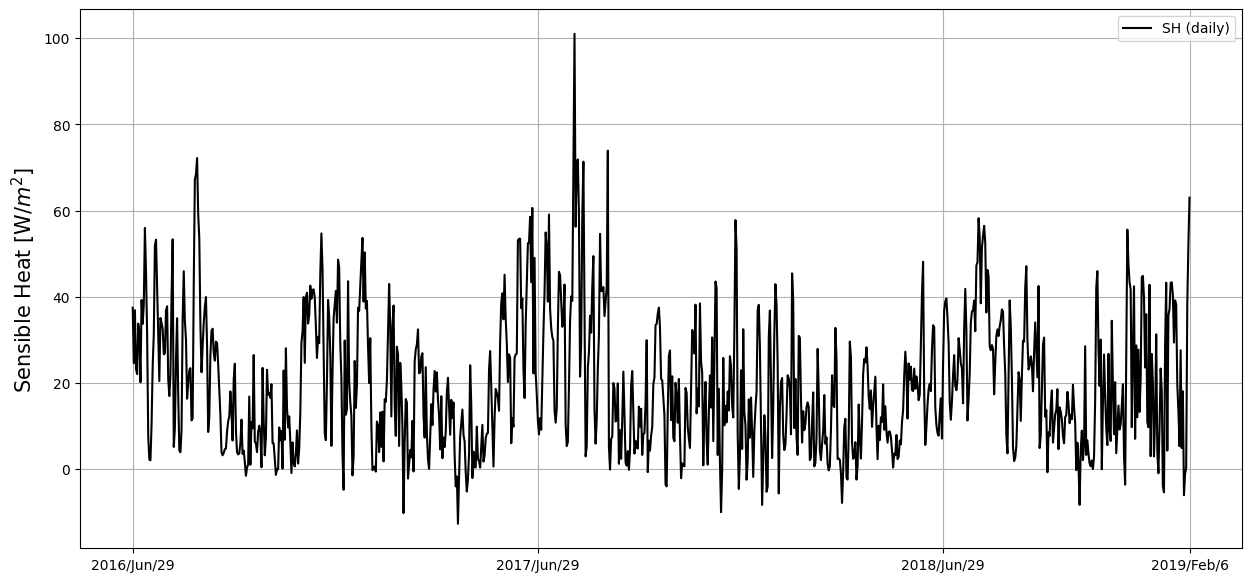
\includegraphics[width=\textwidth]{Immagini/sensibleHeatYear.png}
    \end{minipage}
    \begin{minipage}{0.5\textwidth}
        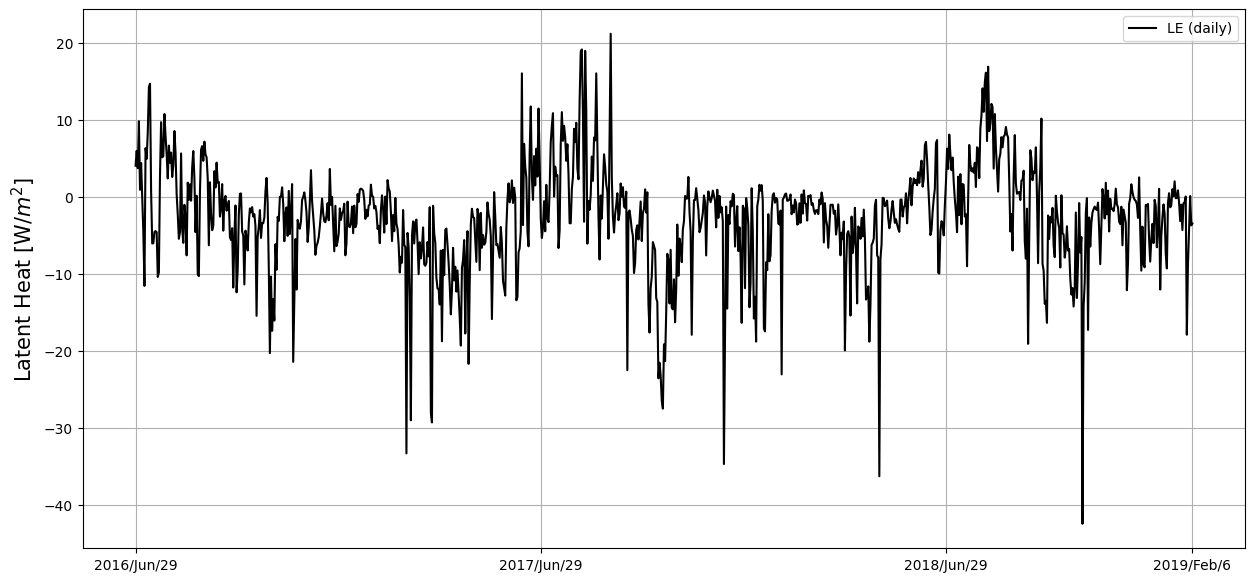
\includegraphics[width=\textwidth]{Immagini/latentHeatYear.png}
    \end{minipage}
  
\end{frame}


\begin{frame}
    \frametitle{Secondo approccio: temperatura superficiale}
    \framesubtitle{}

    \begin{figure}
        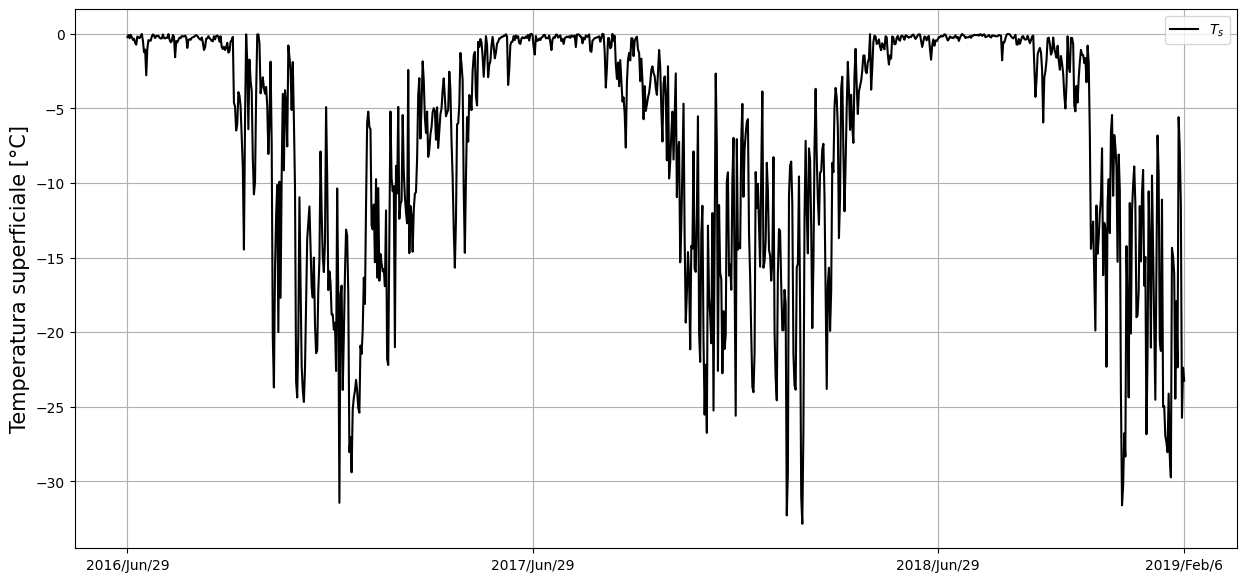
\includegraphics[width=0.9\textwidth]{Immagini/tSupAlt.png}
        \caption{Dati da Oerlemans}
    \end{figure}
  
\end{frame}


\begin{frame}
    \frametitle{Secondo approccio: sensible e latent heat flux}
    \framesubtitle{}

    \center
    \begin{minipage}{0.5\textwidth}
        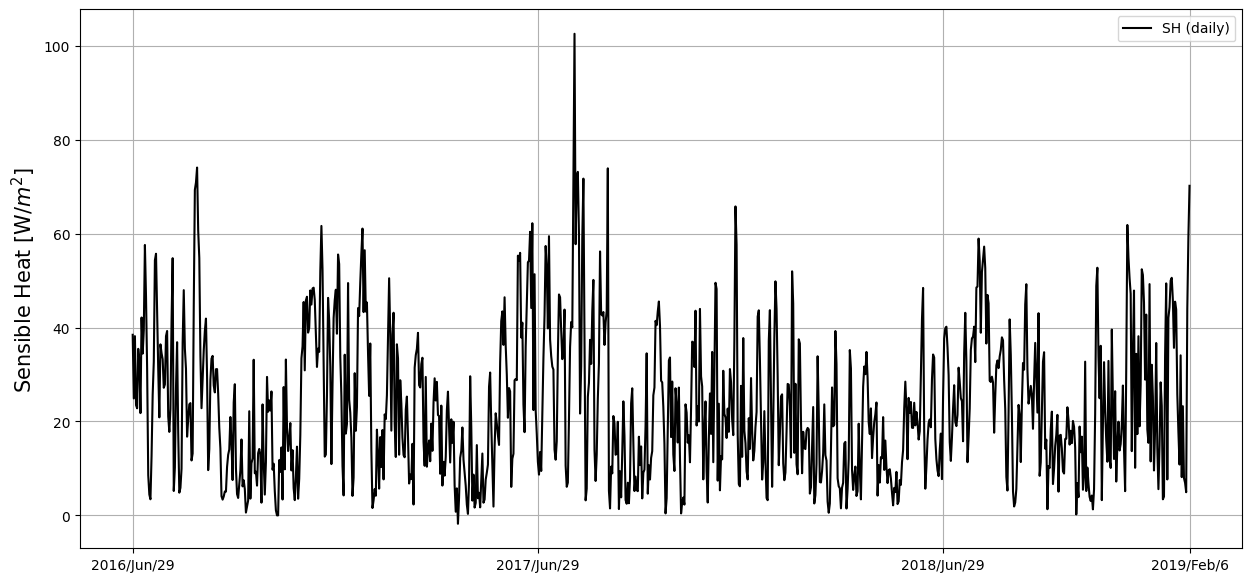
\includegraphics[width=\textwidth]{Immagini/sensibleAlt.png}
    \end{minipage}
    \begin{minipage}{0.5\textwidth}
        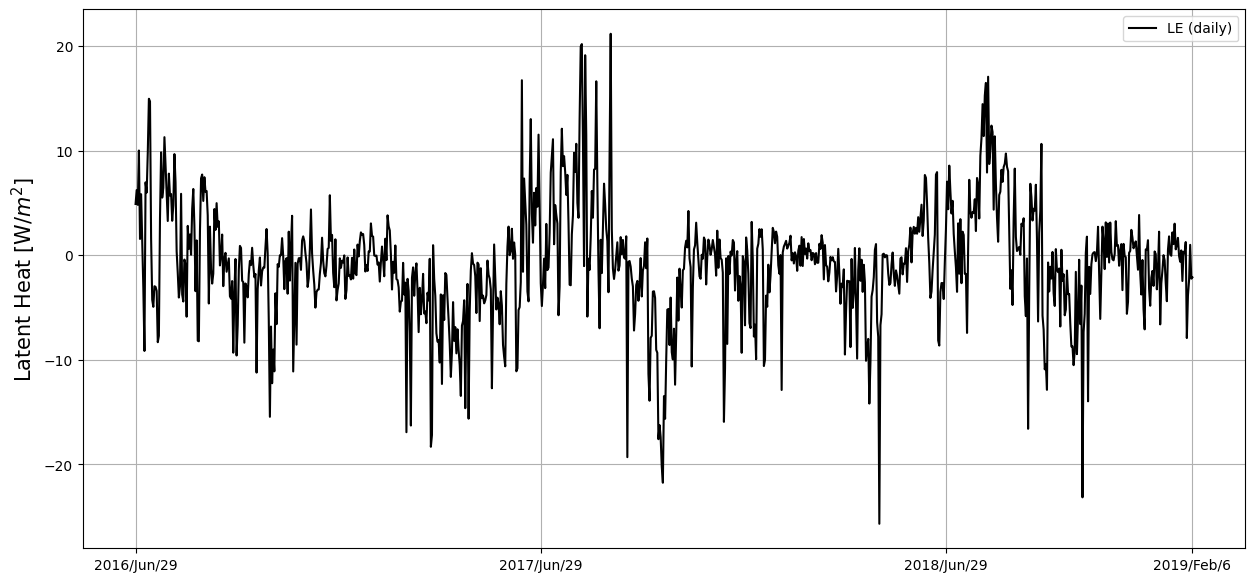
\includegraphics[width=\textwidth]{Immagini/latentAlt.png}
    \end{minipage}

\end{frame}


\begin{frame}
    \frametitle{Secondo approccio: budget energetico}
    \framesubtitle{}

    \begin{figure}
        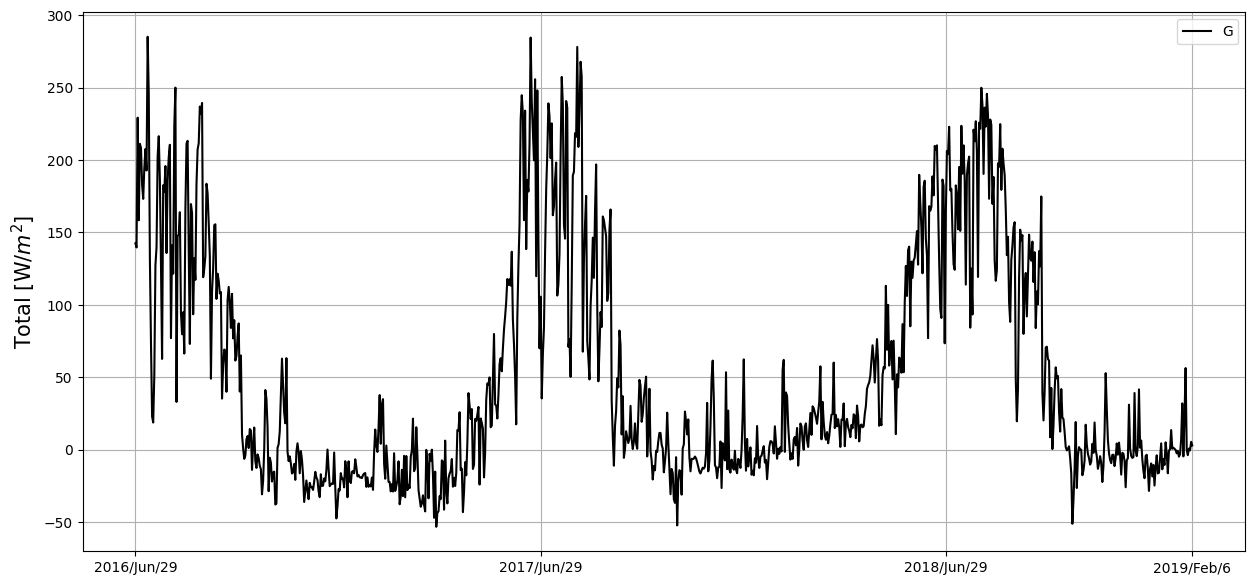
\includegraphics[width=0.9\textwidth]{Immagini/totalAlt.png}
        \caption{Dati da Oerlemans}
    \end{figure}
  
\end{frame}


\begin{frame}
    \frametitle{Secondo approccio: confronto fra modello e misurazioni}
    \framesubtitle{}

    \begin{figure}
        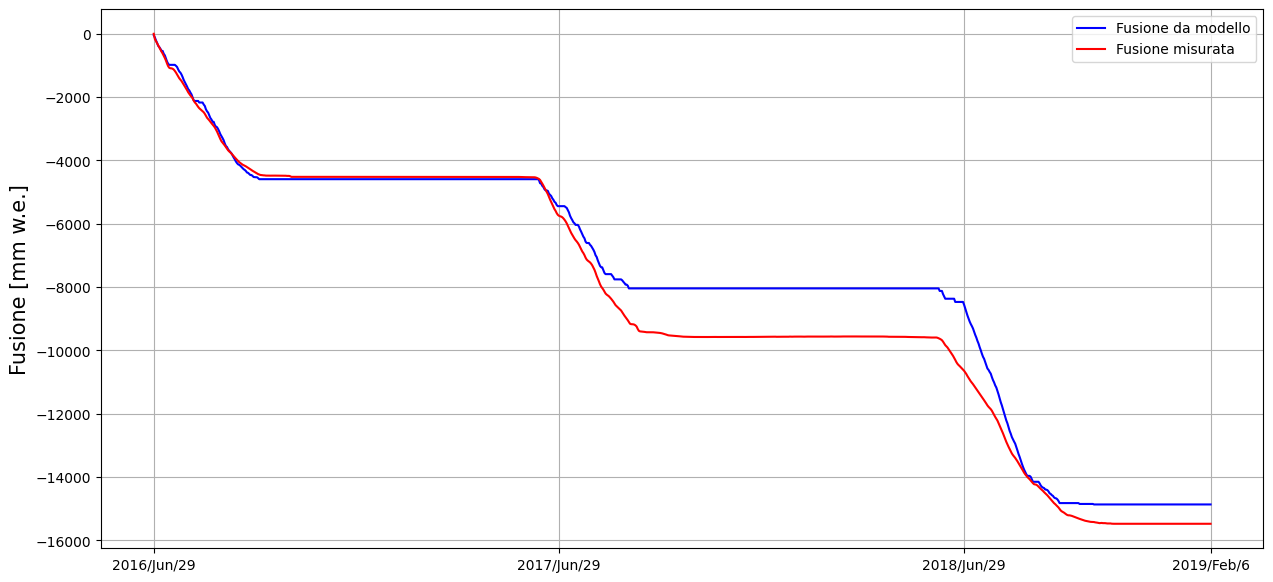
\includegraphics[width=0.9\textwidth]{Immagini/fusioneAlt.png}
        \caption{Dati da Oerlemans}
    \end{figure}
  
\end{frame}

\end{document}